\documentclass[a4paper, 12pt]{article}
\usepackage{fancyhdr}
\usepackage[12pt]{moresize}
\usepackage[pdftex]{graphicx}
\usepackage{epstopdf}
\title{mm20b052.tex}
\author{Roshan Biju mm20b052}
\date{June 2021}
\pagestyle{empty}
\addtolength{\oddsidemargin}{-0.8in}
\addtolength{\evensidemargin}{-1in}
\addtolength{\textwidth}{1.9in}
\addtolength{\topmargin}{-1in}
\addtolength{\textheight}{1.9in}
\begin{document}
\begin{center}
	{\LARGE {\textbf {MM2090 ASSIGNMENT-4}}}
\end{center}

\section{Student Information}
\textbf {Name} : \textbf{\textit {Roshan Biju}}\\
\textbf {Roll No.} : \textbf{\textit {MM20B052}}\\
\textbf {Group} : \textbf{\textit {Group-1}}
\section{MASS-ENERGY EQUIVALENCE EQUATION}
\subsection{EQUATION}
\begin{equation}
	{\LARGE{\textbf{$E=M(C^2)$}}}
	\label{eq:1}
\end{equation}
{\normalsize {Equation \ref{eq:1}  has terms \textbf{E} ,\textbf{M} ,\textbf{C}.}}

{\normalsize { In this equation,}\\
{\normalsize {\textbf{E}\ -Energy of the system}}\\
{\normalsize {\textbf{M}\ -Mass of the system}}\\
{\normalsize {\textbf{C}\ -Speed of light}}
\subsection{DESCRIPTION}

{\small {This equation is the last part of the derivation of Albert Einstien's Special Theory of Relativity.}}

{\small {In physics, mass–energy equivalence is the relationship between mass and energy in a system's rest frame, where the two values mass and energy differ only by a constant and the units of measurement.\\
\\
\ The formula defines the energy E of a particle in its rest frame as the product of mass (m) with the speed of light squared ($c^2$). Because the speed of light is a large number in everyday units ($approximately\ 3x10^8\ meters per second$), the formula implies that a small amount of rest mass corresponds to an enormous amount of energy, which is independent of the composition of the matter

In physical theories prior to that of special relativity, mass and energy were viewed as distinct entities. Furthermore, the energy of a body at rest could be assigned an arbitrary value. In special relativity, however, the energy of a body at rest is determined to be $mc^2$. Thus, each body of rest mass m possesses $mc^2$ of “rest energy,” which potentially is available for conversion to other forms of energy.\\
\\
 This is particularly true in the case of nuclear fusion($fig-2$) reactions that transform hydrogen to helium, in which 0.7 percent of the original rest energy of the hydrogen is converted to other forms of energy. Stars like the Sun shine from the energy released from the rest energy of hydrogen atoms that are fused to form helium.\\
 \\

This equation greatly helped in knowing and quantifying the energy released during all nuclear processes such as fission fusion and radioactive decay,which then led to the discovery of atomic bombs.\\
\\
\begin{figure}
	\centerline{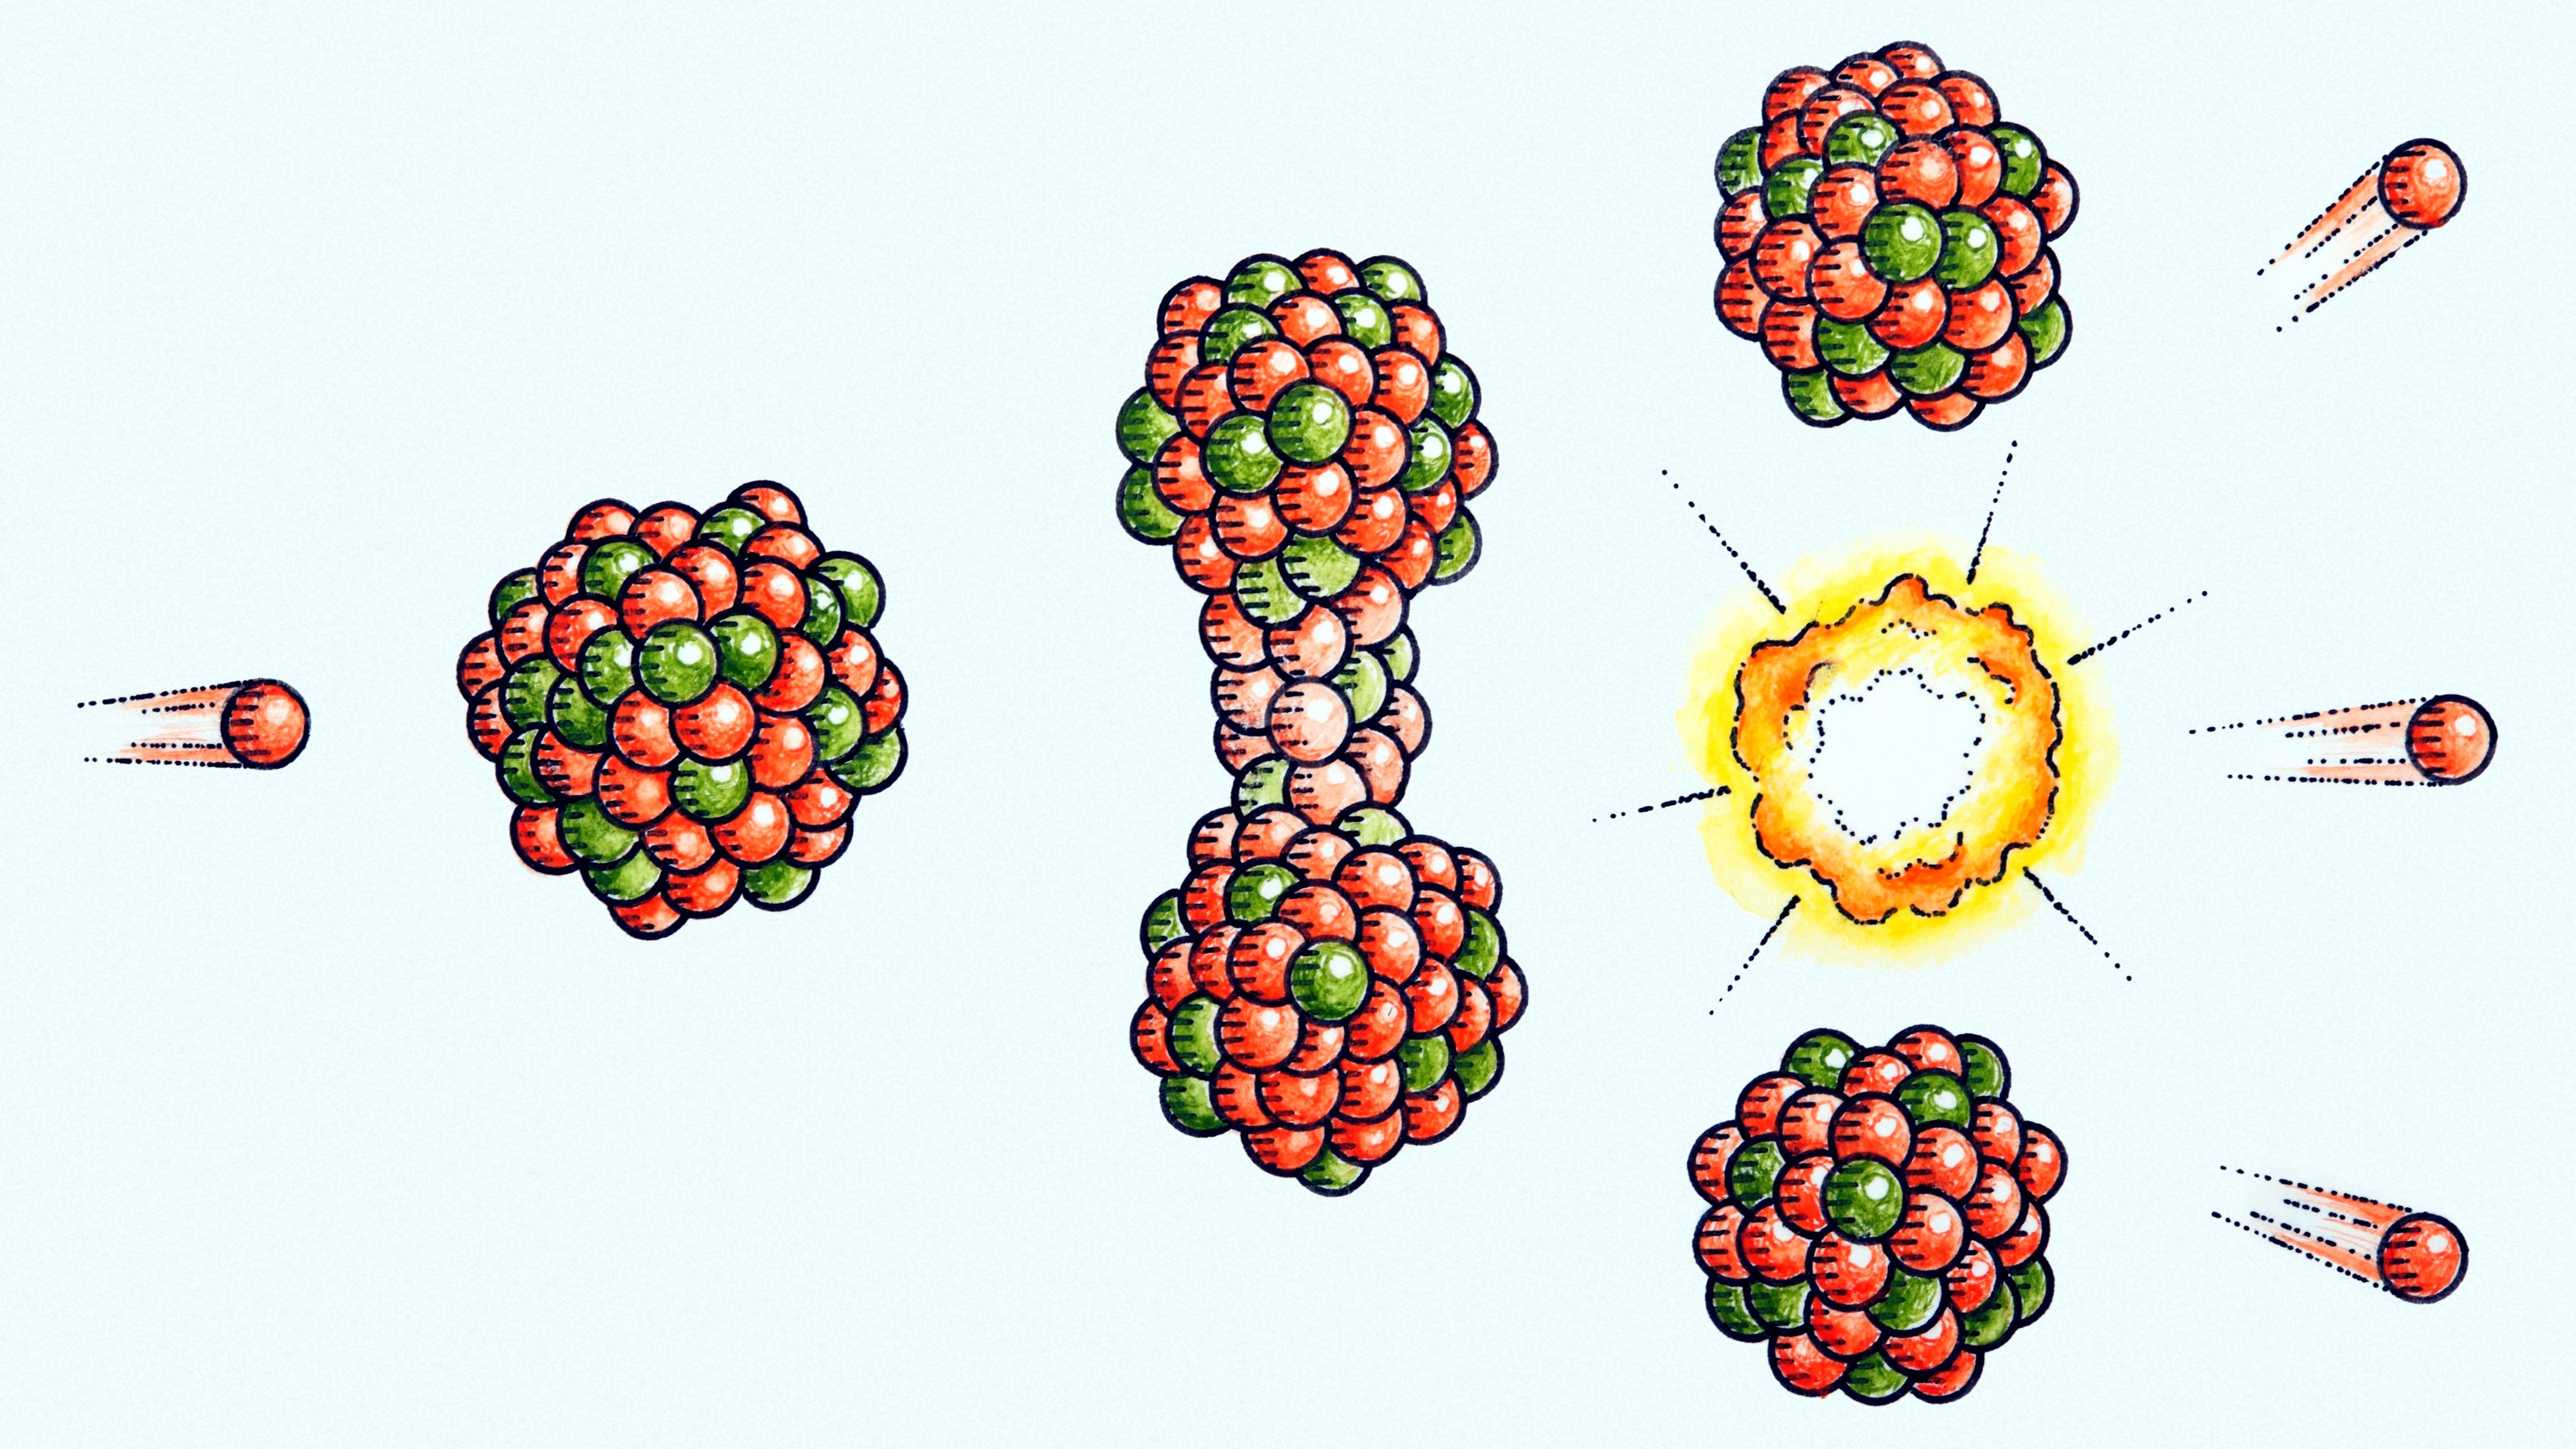
\includegraphics[scale=0.06]{mm20b052(1).jpg}}
		\caption{Atomic fission\cite{fig-1}}
        \label{fig:1}
 \end{figure}
 \begin{figure}
    \centerline{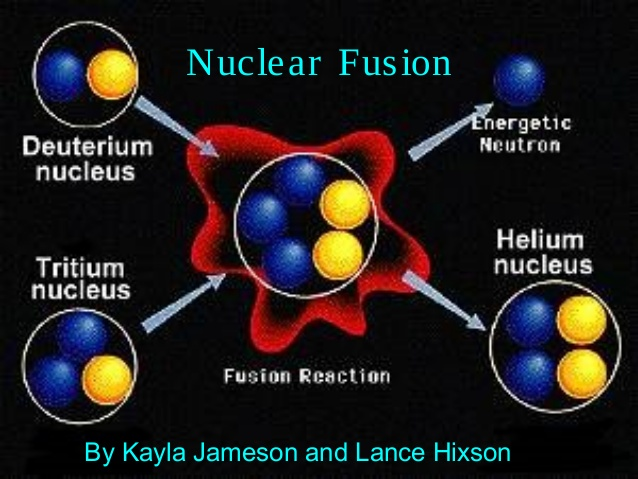
\includegraphics[scale=0.4]{mm20b052(2).jpg}}
        \caption{Atomic fusion\cite{fig-2}}
        \label{fig:2}
\end{figure}

\\
\\

 $links & websites$ \cite{info} \cite{info2}\\ \\ \\ \\

%\bibliographystyle{plain}
%\bibliography{bibliorapy.bib}
}}


\end{document}
